% Import the document class:
\documentclass[conf]{new-aiaa}

% Import packages:
\usepackage{float}
\usepackage{graphicx}
\usepackage{amsmath}
\usepackage{mathtools}
\usepackage{bm}
\usepackage{subfigure}

\usepackage{wrapfig}

% Import packages for debugging:
\usepackage{xcolor}

% Setup:
\graphicspath{{figs/}}
\setcounter{MaxMatrixCols}{20}

% Title:
\title{A Comparison of Indirect Gradient Descent and Single Shooter Methods for Fuel Optimal Time-Fixed Spacecraft Rendezvous}

% Authors:
\author{
  Chris Gnam\footnote{Ph.D Candidate, Department of Aerospace Engineering.  UB ID: 50083665, UBIT: crgnam}
}

%%%%%%%%%%%%%%%%%%%%%%
%%% BEGIN DOCUMENT %%%
%%%%%%%%%%%%%%%%%%%%%%
\begin{document}
\maketitle{}

\begin{abstract}
    Fuel optimal rendezvous and docking can improve mission performance by increasing margin of success and allowing for increased payload capacity.  While an optimal open-loop control law can be found, the final operations conducted during docking of two spacecrafts requires extreme precision and so a feed-back control law is required.  We present here a two stage operation whereby an optimal open-loop control is utilized for rendezvous, bringing the two spacecraft to close proximity at which point an Linear Quadratic control scheme is utilized in conjunction with an Extended Kalman Filter for final docking operations.  The optimal open-loop control law is found for the time-fixed rendezvous problem using a gradient descent numerical approach.  The performance is then demonstrated via a simulated rendezvous and docking scenario with the International Space Station.
\end{abstract}

\tableofcontents
\newpage


%%%%%%%%%%%%%%%%%%%%
%%% Introduction %%%
%%%%%%%%%%%%%%%%%%%%
\section{Introduction}
{\color{red} Discuss the background of rendezvous and docking, and importance of fuel optimal control.  Also outline the basic terminology such as target/chaser vehicle}

\subsection{Existing approaches}
{\color{red} Literature review will go here.  Major ones I want to focus on are:
\begin{itemize}
    \item Guidance and Control for Multi-stage Rendezvous and Docking Operations in the Presence of Uncertainty \cite{jewison}
    \item Optimal Rendezvous Guidance using Linear Quadratic Control \cite{moon}
\end{itemize}
}

\subsection{Proposed Methodology}
In order to achieve both a fuel optimal control as well as to achieve the necessary accuracy required by the spacecraft during docking, we break the flight into two distinct phases.  The first is the rendezvous phase where an open-loop, fuel optimal, time-fixed control scheme will bring the chaser spacecraft to a location 500 meters above the target spacecraft in the Radial direction.  Once this terminal condition is met, the control scheme will transition to an Linear Quadratic based control, providing closed-loop control where an Extended Kalman Filter (EKF) is used to provide estimates of the relative position, velocity, attitude and angular rate between the target and chaser vehicles.


%%%%%%%%%%%%%%%%%%%%%%%%%%%%
%%% Scenario Description %%%
%%%%%%%%%%%%%%%%%%%%%%%%%%%%
\section{Scenario Description}
In this work we explore a simplified resupply mission to the International Space Station (ISS).  This scenario consists of chaser vehicle which is placed into the same orbital plane as the ISS (the target vehicle), but several thousand kilometers behind in the along-track direction.  The vehicle will then

\subsection{Rendezvous and Docking Requirements for the International Space Station}
{\color{red}Discuss the requirements for docking precision, flight time and other things related to nominal ISS proximity operations}\cite{iss}

\subsection{Thrusters}
The chaser vehicle will be the only one of the two vehicles capable of maneuvering, and it will have 6 thrusters located on each of its 6 body axes.  {\color{red} Minimum allowable thrust?  Impulsive thrust or low-continuous thrust?}

\subsection{Sensors and Attitude Control}
The sensors used in the estimation of the relative states are a set of Ultra-Wideband (UWB) transceivers.  These are small modules located on both the target and the chaser vehicle and provide precision ranging.  The sensors are arranged around the docking ports of each spacecraft, and will provide ranges between all pairs of transceivers from one spacecraft to the other.  These range measurements will be fed into the Extended Kalman Filter for state estimation.

For the purposes of this problem, we are only concerning ourselves with the optimal control for the orbital trajectory, and so we are assuming that perfect attitude stabilization of each spacecraft is achieved.  That is, both spacecraft are assumed to hold a nadir pointing attitude throughout the duration of the rendezvous and docking operations.  This will ensure that the 6 thrusters described previously, are aligned with the Radial, Cross-track, and Along-track axes of the Local Vertical Local Horizontal (LVLH) frame as shown in \ref{fig:lvlh}
\begin{figure}[H]
    \centering
    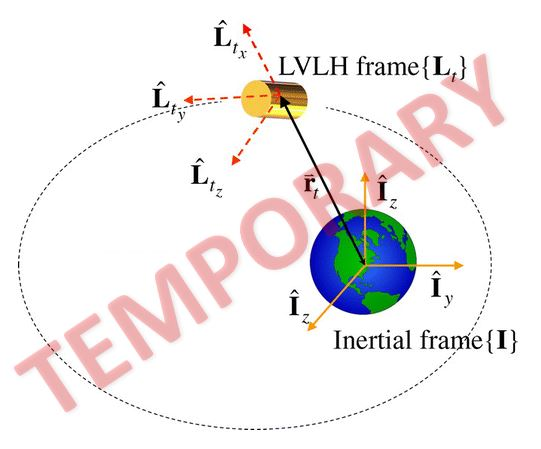
\includegraphics[width=.5\textwidth]{lvlh.JPG}
    \caption{The definition of the LVLH frame, along with the 6 thrusts aligned with the frame.}
    \label{fig:lvlh}
\end{figure}




%%%%%%%%%%%%%%%%%%%%%%%%%%%%%%%%%%%
%%% Ground Truth Dynamics Model %%%
%%%%%%%%%%%%%%%%%%%%%%%%%%%%%%%%%%%
\section{Ground Truth Dynamics Model}
\subsection{Two-body Orbital Motion with Atmospheric Drag}
For both the optimization of the closed-loop control law, as well as for the final demonstration of the overall system performance, we need a dynamics model to simulate ground truth.  For the purposes of this project, we will only be considering two-body orbital motion with atmospheric drag.  For each spacecraft the orbital state is defined as
\begin{equation}\bm x=\begin{bmatrix}\bm r \\ \dot{\bm r}\end{bmatrix}\end{equation}
and the equation of motion is given by
\begin{equation}\ddot{\bm r}=-\frac{\mu}{||\bm r||^3}\bm r + \bm a_d + \bm a_t\label{eq:twobody}\end{equation}
where $\mu = 3.986\times10^{14}$ m$^3$s$^{-2}$ is the gravitational parameter for the Earth, $\bm a_d$ is the force due to atmospheric drag, and $\bm a_t$ is the applied thrust control input.  While perturbations due to the non-uniform geopotential model of the Earth are considerable (notably $J_2$ nodal precession), we are justified in excluding these effects because both the target and chaser vehicle will be at roughly the same altitude and in the same orbital plane.  This will make the effect of this kinds of perturbations negligible when one vehicle's orbit is considered relative to the others.

\subsubsection{Atmospheric Drag Model}

\subsubsection{Thruster Impulse Model}

\subsection{Conversion to LVLH Frame}
The estimated states are the relative coordinates based on the CW equations, which have their definition in the LVLH frame {\color{red} need citation for this}, which is also the frame which the spacecraft body frame (and thus its thrusters) will be aligned with.  As such, the analysis of the orbit determination and control performance will be done using the aforementioned radial, cross-track and along-track coordinates will be used.  The radial direction ($\bm u_r$) is the direction from the center of the Earth to the spacecraft, the along-track direction ($\bm u_w$) is the projection of the velocity vector direction on the plane perpendicular to the radial direction, and the cross-track direction ($\bm u_s$) completes the right-handed coordinate system and points perpendicular to the projected velocity vector and radial direction.  These coordinates are defined as \cite{vallado}
\begin{subequations}\begin{gather}\bm u_r=\frac{\bm r}{||\bm r||} \\ \bm u_w=\frac{\bm r \times \dot{\bm r}}{||\bm r \times \dot{\bm r}||} \\ \bm u_s=\bm u_w \times \bm u_r\end{gather}\end{subequations}





%%%%%%%%%%%%%%%%%%%%%%
%%% Control Scheme %%%
%%%%%%%%%%%%%%%%%%%%%%
\section{Control Scheme}
\subsection{Rendezvous via an Open-loop Control Law}
As stated previously, the proposed methodology include breaking the problem into two separate phases: rendezvous and docking.  A formulation for both the open-loop and closed-loop control laws are outlined here

{\color{red} also need to figure out where to cite Kirk\cite{kirk}}

{\color{red} The problem is a time-fixed optimal control problem, whereby the amount of time required to transition from the initial state to the final state is pre-determined and fixed.  We aim to minimize the total actuation cost, in other words we have a cost function given by
\begin{equation}
    \int_0^{t_f} \left(\bm u^T \bm u\right) dt
    \label{eq:J}
\end{equation}
}

\subsubsection{Initial Control Guess}
{\color{red}
In order to see the optimization process correctly, a reasonable initial guess to the control signal is required.  For this, we have analytically derived 3 separate orbital maneuvers.  The first two being orbital phasing maneuvers to close the in-track distance between the chaser and target vehicles, and the third to send the chaser vehicle into an elliptical orbit with a raise apoapsis, sending it into a elliptical relative orbit, allowing it to achieve the desired final state.
}

\subsubsection{Gradient Descent}

\subsubsection{Single Shooter}



%%%%%%%%%%%%%%%%%%%%%%%%%%
%%% Docking Operations %%%
%%%%%%%%%%%%%%%%%%%%%%%%%%
\subsection{Docking via a Closed-loop Control Law}
\subsubsection{Relative Orbital Motion via Clohessy-Wiltshire Equations}
The Clohessy-Wiltshire (CW) equations are a first order approximation of orbital relative motion.  They make the assumption that the chief spacecraft is in a circular orbit.  The CW equations are particularly useful for rendezvous and docking, or any proximity operations where the deputy and chief spacecraft are in close proximity.  This makes them are an ideal choice for this filtering example.  Given a relative position of the deputy spacecraft of $\left[x,y,z\right]^T$ in a chief-centered coordinate system, the equations of motion of the deputy are given by \cite{vallado}
\begin{subequations}\begin{align}
\ddot {x} &=  3n^{2}x+2n{\dot {y}}\\
\ddot {y} &= -2n{\dot {x}}\\
\ddot {z} &= -n^{2}z
\end{align}\end{subequations}
where $n$ is the mean motion given by
\begin{equation}
    n =\sqrt {\frac {\mu }{a^{3}}}
\end{equation}
where $a$ is the semimajor axis of the chief's orbit and $\mu = 398,600.4~ \textnormal{km}^3\textnormal{s}^{-2}$ is Earth's gravitational parameter.

\subsubsection{Extended Kalman Filter for State Estimation}
{\color{red} NEED TO MAKE THIS FLOW and CITE\cite{me}, \cite{markley}}
An Extended Kalman Filter (EKF) is used to filter the measurements and provide estimates of the relative position, velocity, attitude, and angular rate between the spacecraft.  An overview of the EKF process is given below.  The dynamics are given by a continuous state model and the measurements are assumed to be discrete in time.
\begin{subequations}\begin{gather}
\dot{\bm x}(t) = {\bm f}({\bm x}(t), {\bm u}(t), t) + G(t){\bm w}(t) \\
\tilde{\bm y} = {\bm h}({\bm x}_k, t) + {\bm v}_k
\end{gather}\end{subequations}
where ${\bm w}(t)$ and ${\bm v}_k$ are zero mean Gaussian white noise processes, then the measurement sensitivity matrix is defined by
\begin{equation}
    \left. H_k\left(\hat{\bm x}_k^-\right) \equiv \frac{\partial {\bm h}}{\partial {\bm x}}\right\vert_{\hat{\bm x}_k^-}
\end{equation}
where $\bm x_k^-$ is the \textit{a priori} state estimate.  Given the \textit{a priori} covariance $P_k^-$ and the measurement covariance $R_k$, the gain is then computed by
\begin{equation}
    K_k = P_k^-H_k^T\left(\hat{\bm x}_k^-\right)\left[H_k\left(\hat{\bm x}_k^-\right)P_k^-H_k^T\left(\hat{\bm x}_k^-\right) + R_k\right]^{-1}
\end{equation}
while the state and covariance updates are given by
\begin{subequations}\begin{gather}
    \hat{\bm x}_k^+ = \hat{\bm x}_k^- + K_k\left[\tilde{\bm y}_k - {\bm h}\left(\hat{\bm x}_k^-\right)\right]\\
    P_k^+ = \left[I - K_k H_k\left(\hat{\bm x}_k^-\right)\right]P_k^-
\end{gather}\end{subequations}
The state and covariance are propagated to the next time step using integration of the continuous dynamics given by
\begin{subequations}\begin{gather}
    \dot{\hat{\bm x}}(t) = {\bm f}(\hat{\bm x}(t),{\bm u}(t),t)\\
    \dot{P}(t) = F(t)P(t) + P(t)F^T(t) + G(t)Q(t)G^T(t)
\end{gather}\end{subequations}
In this case, the states to be estimated are given by
\begin{equation}
    \bm{x} \equiv \left[\bm{r}^T \bm{v}^T \bm{\alpha}^T \bm{\omega}^T \right]^T
\end{equation}
which correspond to the relative position vector between the spacecraft in the chief-centered frame, $\bm r = [x\ \ y\ \ z]^T$; the relative velocity vector between the spacecraft, $\bm v = [\dot{x}\ \ \dot{y}\ \ \dot{z}]^T$; the relative attitude between the spacecraft, $\bm\delta\bm\alpha$ defined using the small-error approximation given by Eq. \eqref{eq:smallangle}; and the relative angular rate between the spacecraft, $\bm \omega$.
\begin{equation}
    A_{DC}=\text{expm}\left\lbrace-[\bm \delta \bm \alpha \times]\right\rbrace \label{eq:smallangle}
\end{equation}
The $F$ and $G$ matrices of the system dynamics are given by
\begin{subequations}
\begin{gather}
    F = \begin{bmatrix}
        0    & 0 & 0    & 1  & 0  & 0 & 0 & 0 & 0 & 0          & 0          & 0\\
        0    & 0 & 0    & 0  & 1  & 0 & 0 & 0 & 0 & 0          & 0          & 0\\
        0    & 0 & 0    & 0  & 0  & 1 & 0 & 0 & 0 & 0          & 0          & 0\\
        3n^2 & 0 & 0    & 0  & 2n & 0 & 0 & 0 & 0 & 0          & 0          & 0\\
        0    & 0 & 0    & 2n & 0  & 0 & 0 & 0 & 0 & 0          & 0          & 0\\
        0    & 0 & -n^2 & 0  & 0  & 0 & 0 & 0 & 0 & 0          & 0          & 0\\
        0    & 0 & 0    & 0  & 0  & 0 & 0 & 0 & 0 & 0          & -\hat{x}_3 & \hat{x}_2\\
        0    & 0 & 0    & 0  & 0  & 0 & 0 & 0 & 0 & \hat{x}_3  & 0          & -\hat{x}_1\\
        0    & 0 & 0    & 0  & 0  & 0 & 0 & 0 & 0 & -\hat{x}_2 & \hat{x}_1  & 0\\
        0    & 0 & 0    & 0  & 0  & 0 & 0 & 0 & 0 & 0          & 0          & 0\\
        0    & 0 & 0    & 0  & 0  & 0 & 0 & 0 & 0 & 0          & 0          & 0\\
        0    & 0 & 0    & 0  & 0  & 0 & 0 & 0 & 0 & 0          & 0          & 0
        \end{bmatrix}\\
    G = I_{12\times12}
\end{gather}
\end{subequations}
The process noise covariance matrix is taken to be {\color{red} (update this for drag perturbation inclusion)}
\begin{equation}
    Q = \begin{bmatrix}
        0_{3\times3} & 0_{3\times3} & 0_{3\times3} & 0_{3\times3}\\ 
        0_{3\times3} & 1\times10^{-6}I_{3\times3} & 0_{3\times3} & 0_{3\times3} \\ 
        0_{3\times3} & 0_{3\times3} & 0_{3\times3} & 0_{3\times3}\\ 
        0_{3\times3} & 0_{3\times3} & 0_{3\times3} & 0_{3\times3}
        \end{bmatrix}
\end{equation}
where the nonzero term in the velocity states accounts for uncertainty in control inputs such as thruster firings as well as the the errors in the linearized CW dynamics.  Measurements are assumed to be only range measurements, and the measurement sensitivity matrix is given by
\begin{equation}H = \begin{bmatrix}\displaystyle\frac{\partial \bm \rho}{\partial \bm r} & \displaystyle\frac{\partial \bm \rho}{\partial \bm v} & \displaystyle\frac{\partial \bm \rho}{\partial \bm \delta\bm\alpha} & \displaystyle\frac{\partial \bm \rho}{\partial \bm \omega}\end{bmatrix}\end{equation}
where the $\frac{\partial\bm\rho}{\partial\bm r}$ and $\frac{\partial \bm \rho}{\partial\bm\delta\bm\alpha}$ terms are given by 
\begin{subequations}
\begin{gather}
    \frac{\partial \rho}{\partial x}=-\frac{\rho_1}{\rho} \\
    \frac{\partial \rho}{\partial y}=-\frac{\rho_2}{\rho} \\
    \frac{\partial \rho}{\partial z}=-\frac{\rho_3}{\rho} \\
    \frac{\partial \rho}{\partial \delta \alpha_1}=-\frac{1}{\rho}(c_3\rho_2-c_2\rho_3) \\
    \frac{\partial \rho}{\partial \delta \alpha _2}=\frac{1}{\rho}(c_3\rho_1-c_1\rho_3) \\
    \frac{\partial \rho}{\partial \delta \alpha_3}=\frac{1}{\rho}(c_2\rho_1-c_1\rho_2)
\end{gather}
\label{eq:partials}
\end{subequations}
and the $\frac{\partial \bm \rho}{\partial \bm v}$ and $\frac{\partial \bm \rho}{\partial \bm \omega}$ terms are zero.


\subsubsection{Linear Quadratic Gaussian (LQG) Control}
For the final phases of the the rendezvous and docking operation, a feedback control loop is required in order to achieve the necessary precision.  Luckily, the relative motion between spacecraft in close proximity is very nearly linear, and so a Linear Quadratic Regulator (LQR) can be used.  Specifically, we have implemented a Linear Quadratic Gaussian (LQG) control scheme, which is a combination of a Kalman Filter and an LQR.  For our specific use case, we will be using an Extended Kalman Filter (EKF) which is outlined in the following section.

{\color{red} Show Linear Quadratic Equations}






%%%%%%%%%%%%%%%%%%%%%%%%%%
%%% Simulation Results %%%
%%%%%%%%%%%%%%%%%%%%%%%%%%
\section{Simulation Results}
\subsection{Gradient Descent Achieved Optimal Rendezvous Control with LQG Docking Control}

\subsection{Single Shooter Achieved Optimal Rendezvous Control with LQG Docking Control}



%%%%%%%%%%%%%%%%%%%%%%%%%%%%%%%%%%%%%%%%%
%%% Optimization of Open-loop control %%%
%%%%%%%%%%%%%%%%%%%%%%%%%%%%%%%%%%%%%%%%%
\section{Comparison in Optimal Open-loop Control Signals}





%%%%%%%%%%%%%%%%%%%
%%% Conclusions %%%
%%%%%%%%%%%%%%%%%%%
\section{Conclusions}




% %%%%%%%%%%%%%%%%%%%%
% %%% BIBLIOGRAPHY %%%
% %%%%%%%%%%%%%%%%%%%%
\bibliography{ref}
			
\end{document}
